%% Beispiel für Klasse tudposter.cls (Version 0.5).
%%
%% Autor: Martin Zabel (martin.zabel@tu-dresden.de)
%%        Tobias schlemmer (tobias.schlemmer@mailbox.tu-dresden.de)
%%
%% Klassenoptionen siehe tudposter.cls.
%%
%%
%% Wir bevorzugen PDFLaTeX. Für den Fall, dass die CD-Schriften nicht
%% in der Standardkonfiguration erwähnt sind laden wir die .map-Datei
%% Wichtig: das muss vor dem ersten Font-Befehl (also vor der
%% Dokumentklasse geschehen.
%
% Diese Zeilen sind jetzt auskommentiert, da dies das Paket „tudfonts“
% jetzt übernimmt
%
%\pdfmapfile{+univers.map}
%\pdfmapfile{+dinbold.map}
%%
\documentclass[serifmath,a0paper,noDIN,Mathematik]{tudmathposter}
\listfiles
% Bei Bedarf: dinBold für Section. Dann aber auch Überschrift nur in
% Großbuchstaben.
%\addtokomafont{section}{\dinBold}

% In diesem Poster benötigte Pakete.
% Jedem wie es beliebt.
\usepackage[T1]{fontenc}
\usepackage[utf8]{inputenc} % latin1 (Linux) oder ansinew (Win) wenn
                            % nicht UTF 8
\usepackage[ngerman]{babel}
\usepackage{multicol}
\usepackage{tikz}
\usepackage{url}
%\usepackage{tabularx}

% Beschriftung im Seitenkopf und Seitenfuß
\institut{Institut für Algebra}
\professur{Professur für \TeX nische Algebra}
\author{T. Schlemmer, M. Behrisch und D. Borchmann}% Zum Beispiel für Kontaktdaten.
\telefon{0351 463-35078}
\fax{0351 463-\dots}
\homepage{\small\url{http://www.math.tu-dresden.de/~schlemme/tudmathposter/}}
\zweitlogofile{mathelogo}

\title{Die Dokumentklasse „tudmathposter“}
\subtitle{Eine \LaTeX klasse für die Evaluationsposter}
\grautabelle
\begin{document}
%\color{HKS41K100}%
%%%%%%%%%%%%%%%%%%%%%%%%%%%%%%%%%%%%%%%%%%%%%%%%%%%%%%%%%%%%%%%%%%%%%%%%%%%%
%%% Poster-Titel
%%%%%%%%%%%%%%%%%%%%%%%%%%%%%%%%%%%%%%%%%%%%%%%%%%%%%%%%%%%%%%%%%%%%%%%%%%%%
\maketitle
%%%%%%%%%%%%%%%%%%%%%%%%%%%%%%%%%%%%%%%%%%%%%%%%%%%%%%%%%%%%%%%%%%%%%%%%%%%%
%%% Poster-Inhalt

\section{Hinweise zur Klasse}
\begin{multicols}{2}%
Die Dokumentklasse „tudmathposter“ wurde für die Vorbereitung von
Postern anlässlich der Evaluation 2010 des Fachbereiches Mathematik
der TU Dresden aufgesetzt. Sie basiert auf der Beispielklasse des
CD-Büros der TUD von Martin Zabel.

\subsection{Aufruf}

{\small\textbackslash
documentclass[noDIN,a0paper,Mathematik]\{tudmathposter\}}

Die Klassenoptionen sind mit anzugeben. Andernfalls fällt die Klasse
in einigen Einstellungen auf das Standard-CD der TUD zurück.
\subsection{Neue Kommandos}
\begin{description}
\item[\textbackslash tudfont\{font\}] wählt eine der Univers-Varianten
  der TUD (siehe Tab. \ref{tab:schriften}aus. Hinweis: Der Schriftschnitt „Univers 45 Light Bold“
  wird nicht mit ausgeliefert, sondern muss durch „Univers 60
  Bold“ ersetzt werden. Es sollte sich kein Problem ergeben.
\item[\textbackslash begin\{farbtabellen\}\dots\textbackslash
  end\{farbtabellen\}]
Innerhalb dieser Umgebung werden alle Tabellen farbig gesetzt ähnlich
Tabelle \ref{tab:schriften}. Die Tabellen müssen in eine angemessene
Tabellenumgebung (vorzugsweise tabularx) eingebettet werden. Es wurde bewusst darauf
verzichtet, eine eigene Umgebung zu definieren, um die Kreativität
nicht weiter zu beschränken.
\item[\textbackslash grautabelle und \textbackslash blautabelle]
  schaltet die Farben für die mehrfarbigen Tabellen um.
\item[\textbackslash color\{HKS$x$K$y$\}, \textbackslash textcolor\{HKS$x$K$y$\} usw.] Diese
  Makros wurden nicht neu definiert, wohl aber die Farben. Sie sind
  den Sonderfarben der HKS-Tabelle nachempfunden. Zur Auswahl stehen
  \[
  x\in\{41,92\}\text{ und } y\in \{10,20,30,40,50,60,70,80,100\}.
  \]
  Dabei
  steht der Wert $100$ für die unveränderte HKS-Farbe (die Farbe des
  CD) und die kleineren Werte sind abgeschwächte Werte für Tabellen,
  Zeichnungen etc. Die genauen Vierfarb-Werte können aus der
  Dokumentklasse entnommen werden. 

  Wenn die Sonderfarben zur Verfügung stehen, sollten wenigstens
  HKS41K100 und HKS92K100 in der PDF-Datei durch spezielle Sonderfarben
  ersetzt werden. Hierbei kann das \LaTeX-Paket spotcolor hilfreich
  sein (ungetestet, daher nicht angeboten).
\end{description}
\end{multicols}

\begin{table}[h]
  \begin{farbtabellen}
    \begin{tabularx}{\linewidth}{|X|X|X|}
      \rowcolor{HKS41K60}\textbf{\color{white}\rule{0pt}{1em}Spaltenüberschrift}&\textbf{\color{white}Spaltenüberschrift}&\textbf{\color{white}Spaltenüberschrift}\\\hline
Univers CE 75 Black&
Univers CE 75 Black Oblique&
Univers CE 60\\
Univers CE 60 Oblique&
Univers CE 45 Light&
Univers CE 45 Light Oblique\\
Univers CE 55&
Univers CE 55 Oblique&
Din Bold
    \end{tabularx}
  \end{farbtabellen}

  \caption{Mögliche Schriftarten für \textbackslash tudfont}
  \label{tab:schriften}
\end{table}

\begin{multicols}2
  \centersubsection{Weitere Makros}
  Eine ganze Reihe von weiteren Kommandos kann benutzt werden, um
  die Üblichen Angaben zu machen. Die Namen sollten selbsterklärend
  sein.

  Es sind \textbackslash title, \textbackslash subtitle,
  \textbackslash einrichtung, \textbackslash fachrichtung,
  \textbackslash institut, \textbackslash professur, \textbackslash
  telefon, \textbackslash \fax, \textbackslash homepage
  
  Ein Beispiel für die Benutzung sehen sie am Anfang dieser .tex-Datei.
  
  Einige dieser Makros sind sinnvoll vorbelegt.
  
  Das Makro
  \textbackslash fusszeile erlaubt es, den gesamten Seitenfuß
  umzudefinieren.
  \centersubsection {Schriften}
  Als Schriften stehen die Univers-Familie, sowie der fette
  Schriftschnitt von Din bereit. Entsprechend der Vorgabe des
  Prodekanates werden die Din-Schriften allerdings nicht
  verwendet. Dies wird über die Option „noDIN“ der Dokumentklasse
  mitgeteilt.

  Als Schriftgrößen stehen die normalen Größen von \textbackslash tiny
  bis \textbackslash Huge zur Verfügung. Dabei wurden zunächst die
  Größen aus der Vorgabe definiert und dann zusätzliche Größen
  interpoliert. Bei Verwendung der Standard-\LaTeX-Makros zur
  Textauszeichnug sollte die Schriftgröße automatisch richtig gesetzt
  werden.
  \enlargethispage{4\baselineskip}
\subsection{Geladene Pakete}
  Die Dokumentklasse basiert auf der Klasse „scrartcl“ aus dem
  KOMA-Skript-Paket. Dieses Paket hat sich als Standardklassen für
  europäischen Textsatz gegenüber den angelsächsischen Standardklassen
  durchgesetzt.

  Weiterhin werden die Pakete „calc“, „xcolor“, „graphicx“,
  „textcomp“, „tabularx“ und „lmodern“ nachgeladen. Es wird empfohlen,
  das Paket „multicols“ zu verwenden.

  \subsection{Team}
  Die Klasse wurde von Mike Behrisch, Daniel Borchmann und Tobias
  Schlemmer angepasst. Die Autoren stehen für Fragen bereit.
\end{multicols}
\pagebreak
\fax{}%
\title{Updates}%
\subtitle{Änderungen an der Klasse für die neue Version}
\maketitle
\section{Version 1.1 (09.\,07.~2010)}
\begin{multicols}2
  \subsection{Fehlerkorrekturen}
 \begin{figurehere}
    \centerline{%
      \fbox{%
        \begin{minipage}{0.9\linewidth}
          \begin{itemize}
          \item In der Klasse wurde der Klassenname korrigiert (Warnung behoben)
          \item Der Fakultätsname wurde korrigiert
          \end{itemize}
        \end{minipage}%
      }%
    }
    \caption{Fehlerkorrekturen}
  \end{figurehere}
  \subsection{Erweiterungen}
  \begin{tablehere}
    \centering
    \begin{farbtabellen}
      \begin{tabular}{||c|p{0.8\linewidth}||}
        \hline\hline
        Nr.&Beschreibung\\\hline\hline
        1&Neue Umgebungen „\textbf{tablehere}“ und „\textbf{figurehere}“ für die Verwendung
        anstelle von Fließobjekten innerhalb von Multicol-Umgebungen\\\hline
        2&Schriftgröße für Tabellen- und Abbildungsunterschriften reduziert.\\\hline
      \end{tabular}
    \end{farbtabellen}
    \caption{Erweiterungen}
  \end{tablehere}
\end{multicols}
\section{Version 1.2 (11.\,07.~2010)}
\begin{multicols}2
\subsection{Korrekturen}
Verbesserter Zeilenumbruch im Fußbereich, wenn nur Telefonnummer oder nur Faxnummer angegeben sind (incl. Demonstration)
\subsection{Erweiterungen}
Demonstration der Nutzung vom Paket „url“ für die Angabe der Homepage
\end{multicols}
\section{Version 1.3 (03.\,08.~2010)}
\begin{multicols}3
\subsection{Korrekturen}
\begin{itemize}
\item Die Schriftgrößen der Matheschriften bei „serifmath“ entsprechen jetzt denen der Univers.
\item Weitere Mathematik-Symbole sind jetzt verfügbar.
\end{itemize}

\subsection{Erweiterungen}
\begin{itemize}
\item Die Fontdefinitionen wurden in eine Datei tudfonts.sty
  ausgelagert, die für andere Projekte (Übungsblätter, Scheine etc.)
  eingebunden werden kann. Diese unterstützt die Optionen „noDIN“ (für 
  Definitionen ohne DIN Bold, „noeulermath“ um die AMS Euler-Schriften
  nicht zu laden und „serifmath“, die die klassischen
  Mathematikschriften aus dem Paket „lmodern“ lädt.
\item tudfonts.sty lädt die AMS Euler-Schriften,
  um Mathematiksymbole darzustellen. \textbf{Dadurch ändert sich das
    Erscheinungsbild der Formeln.} Das alte Verhalten kann
  (verbessert) mit der Option „noeulermath“ wiederhergestellt werden.
\item Neue Makros \textbf{\textbackslash tudmathsizefactor} und
  \textbf{\textbackslash DeclareTudMathSizes}. Ersteres stellt das
  Verhältnis zwischen Matheschriftgröße und Brotschrift dar
  (Voreinstellung: „7/6“ für „serifmath“ und sonst „1“). Es kann mit
  \textbackslash renewcommand umdefiniert werden. Das zweitere bekommt
  vier Argumente, eine Brotschriftgröße und drei Mathematikgrößen. Die
  erste der Mathematikgrößen sollte der Brotschriftgröße (also der
  normalen Schriftgröße) entsprechen. Die anderen beiden sind
  entsprechend den Einstellungen kleiner zu wählen.
\item Neues Paket „rescalefonts.sty“. Damit werden Schriftgrößen
  umgerechtnet. Das Makro \textbf{\textbackslash fontscaling{\textit{Faktor}}}
  legt den Umrechnungsfaktor fest. Beispielsweise bewirkt
  „\textbackslash fontscaling\{3\}“, dass für eine $30$\,pt"=Schrift
  aus der LM-Familie lmr10 geladen wird. Dieses Paket wird automatisch
  mit dem Faktor 3 geladen.
\item Das „DRESDEN Concept“-Logo wurde integriert.
\item Neue Makros \textbf{\textbackslash zweitlogo},
  \textbf{\textbackslash zweitlogofile}, \textbf{\textbackslash
    drittlogo} und \textbf{\textbackslash drittlogofile}, mit denen
  das Zweit- (Instituts-) und das Drittlogo („DRESDEN Concept“)
  eingestellt werden können. Die Variante mit „\dots file“ ist jeweils
  für den Dateinamen der entsprechenden PDF-Datei vorgesehen (ohne
  Endung „.pdf“), während die kürzere Variante beliebigen LaTeX-Code
  aufnehmen kann, wenn das Logo komplizierter dargestellt werden muss.
\end{itemize}
\end{multicols}
\pagebreak
\fax{nur Tel.: 0351 463-35078}%
\title{Beispiel}%
\maketitle
\centersubsection{Überschrift 2}

\begin{farbtabellen}
\begin{tabularx}{\linewidth}{|X|X|X|}
\hline
Lorem ipsum dolor sit amet, conse&
Lorem ipsum dolor sit amet, conse&
Lorem ipsum dolor sit amet, conse\\\hline
Lorem ipsum dolor sit amet, conse&
Lorem ipsum dolor sit amet, conse&
Lorem ipsum dolor sit amet, conse\\\hline
Lorem ipsum dolor sit amet, conse&
Lorem ipsum dolor sit amet, conse&
Lorem ipsum dolor sit amet, conse\\\hline
\end{tabularx}
\end{farbtabellen}

\vspace{93.1pt}
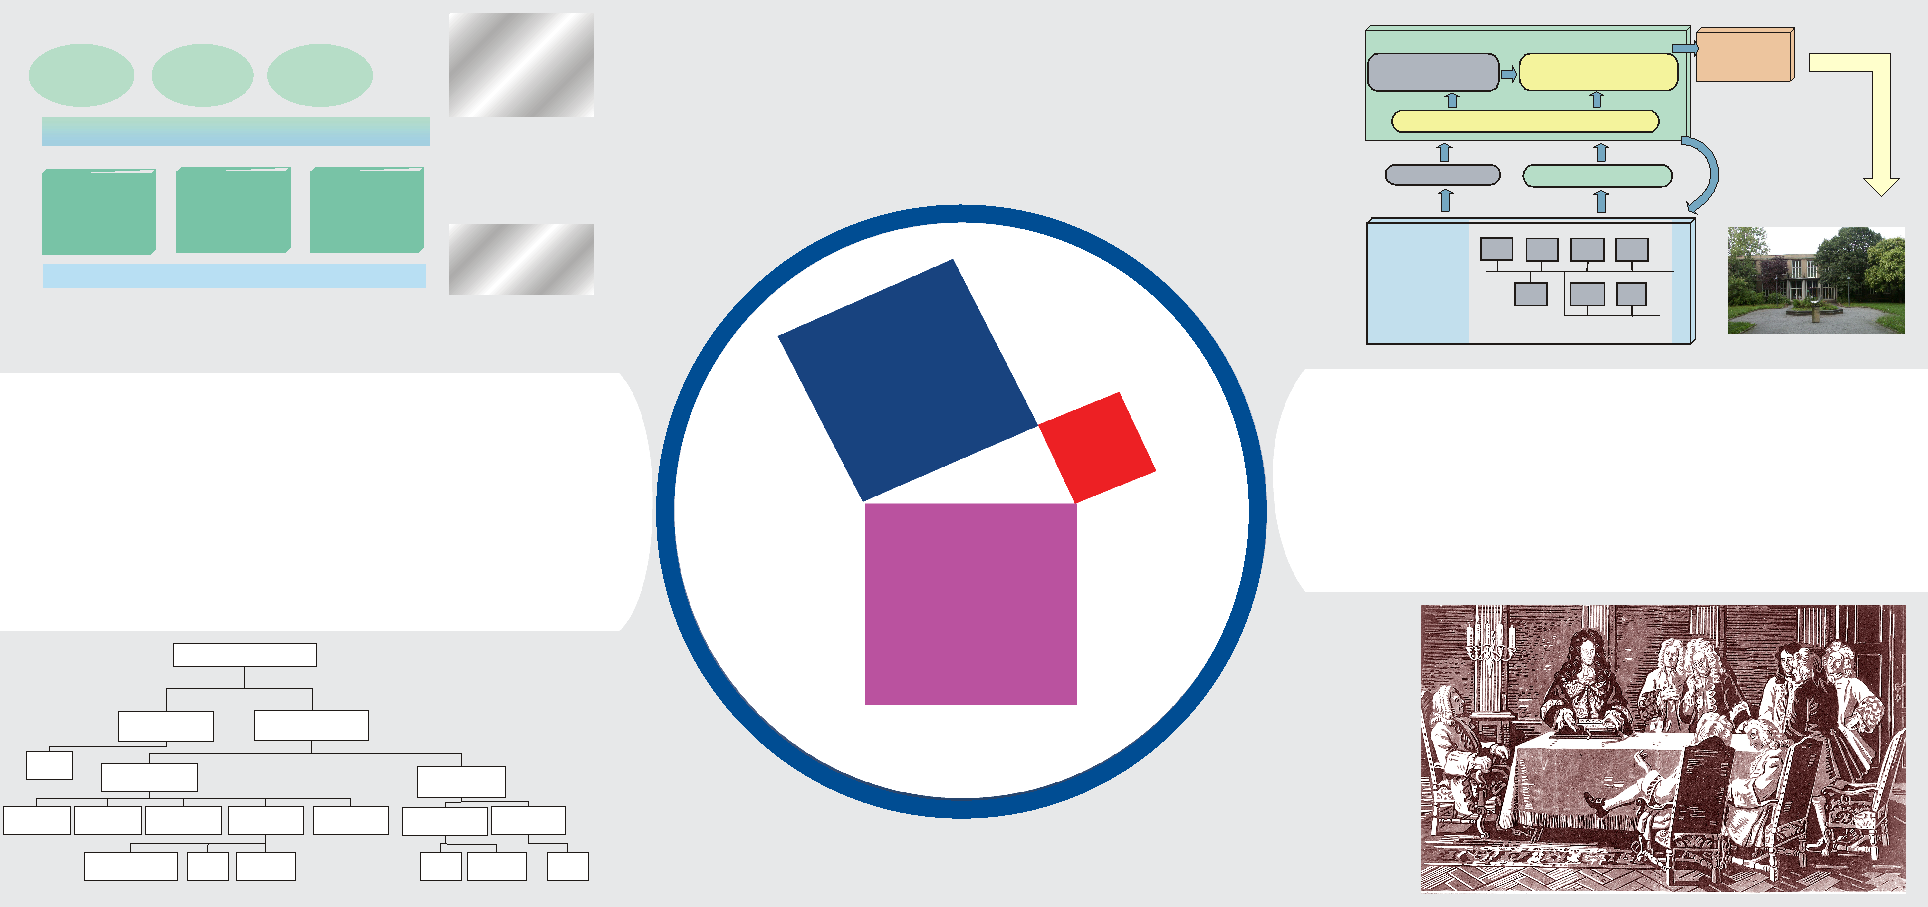
\includegraphics[width=\linewidth]{image2.png}
\centersection{Ausblick}

\begin{multicols}{2}
Auch Matrizen können unterschiedlich gefärbte Zeilen bekommen (müssen
aber nicht):\\\strut
\end{multicols}
\[
p^2=+\begin{pmatrix} a_1 &a_2\\a_3&a_4\end{pmatrix} = 
\begin{farbtabellen}\begin{pmatrix} a_1 &a_2\\a_3&a_4\end{pmatrix}\end{farbtabellen}
\]
\begin{multicols}{2}
  Lorem ipsum dolor sit amet, consectetuer adipiscing elit, sed diam nonummy nibh euismod tincidunt ut laoreet dolore Lorem ipsum dolor sit amet, consectetuer adipiscing elit, sed diam nonummy nibh euismod tincidunt ut laoreet dolore magna aliquam Lorem ipsum dolor sit amet, consectetuer adipiscing elit, sed diam nonummy nibh euismod tincidunt ut 
\end{multicols}
\pagebreak
\homepage{http://www.math.tu-dresden.de/\textasciitilde schlemme/tudmathposter/}
\telefon{}%
\title{2. Plakat}%
\subtitle{testausgaben}%
\maketitle
\section*{Test Aufzählung}
\begin{multicols}{2}
Dies ist eine Aufzählung.

\begin{itemize}
\item Item
\item Item
  \begin{itemize}
  \item SubItem
  \item SubItem
  \item SubItem
  \end{itemize}
\item Item
\item Item
\item Item
\item Item
\item Item
\item[\raisebox{.2ex}{$\Rightarrow$}] Ergebnis
\end{itemize}

\section*{Test Buchstaben / Zahlen}
A B C D E F G H I J K L M N O P Q R S T U V W X Y Z Ä Ö Ü.
a b c d e f g h i j k l m n o p q r s t u v w x y z ä ö ü ß.
0 1 2 3 4 5 6 7 8 9.

\section*{Test Unterabschnitte}
\subsection*{Unterabschnitt 1}
Dies ist ein Absatz.
\subsection*{Unterabschnitt 2}
Dies ist ein noch ein Absatz.

\vfill
%\columnbreak
\section*{Test Mathematisches}
Vergleich Schriftart in Text und Formel:\\
1+2=3 vs. $1+2=3$.

Abgesetze Formeln:
\begin{eqnarray}
\mbox{Gleichung:}&&1+2*3-4/5\approx6\\
\mbox{Funktion:}&&A(r)=\pi r^2\\
\mbox{Funktionsnamen:}&&\lim_{n\to0}\frac{1}{n}=\infty\\
\mbox{Summensymbol:}&&e=\sum_{k=0}^{\infty}\frac{1}{k!}\\
\text{w$e$iter:}&&\int\limits_0^\pi \sin x\,dx = 2
\end{eqnarray}
a$a$a b$b$b c$c$c d$d$d e$e$e f$f$f g$g$g h$h$h i$i$i j$j$j k$k$k
l$l$l m$m$m n$n$n o$o$o p$p$p q$q$q r$r$r s$s$s t$t$t u$u$u v$v$v
w$w$w x$x$x y$y$y z$z$z 1$1$1 2$2$2 3$3$3 4$4$4 5$5$5 6$6$6 7$7$7
8$8$8 9$9$9 0$0$0 A$A$A B$B$B C$C$C E$E$E F$F$F G$G$G H$H$H I$I$I
J$J$J K$K$K L$L$L M$M$M N$N$N O$O$O P$P$P Q$Q$Q R$R$R S$S$S T$T$T
U$U$U V$V$V W$W$W X$X$X Y$Y$Y Z$Z$Z $R\mathbb RR$ $\partial x$
$G\Gamma D\Delta T\Theta L\Lambda X\Xi P\Pi S\Sigma Y\Upsilon F\Phi
Ps\Psi O\Omega s\sigma r\rho$ 
\[
\mathbf{\frac{\text{A}ABCDEFGHI\mathfrak{JKLM}NOPQRSTUVWXYZ\text{Z}}
{\text{a}abcdefghijklmnopqrstuvwxyz\text{z}}}
\]
$!$!$($($)$)$+$+$-$-$=$=$[$[$]$]$"$"$\&$\&$:$:$;$;$?$?$`$`$|$|
$\aleph\Re\Im\neg=\neq\wedge\vee\setminus\sim\mid\mathsection$
$\intop\ointop\braceld\bracerd\bracelu\braceru\infty\nearrow\searrow\nwarrow\swarrow$
$\Leftrightarrow\Leftarrow\Rightarrow\leftrightarrow\rightarrow\leftharpoonup\leftharpoondown$

\vfill
%\columnbreak
\section*{Test Grafik}
\rule{\linewidth}{2cm}
\end{multicols}

\begin{multicols}{2}
\makeatletter
\@tempdima=1cm
1cm = $\the\@tempdima$\\
\makeatother
topmargin = $\the\topmargin$\\
headheight = $\the\headheight$\\
headsep = $\the\headsep$\\
topskip = $\the\topskip$\\
baselineskip = $\the\baselineskip$\\
footskip = $\the\footskip$\\
{\textcolor{black}{
textheight = $\the\textheight$}}\\
oddsidemargin = $\the\oddsidemargin$\\
evensidemargin = $\the\evensidemargin$\\
textwidth = $\the\textwidth$\\
paperheight = $\the\paperheight$\\
paperwidth = $\the\paperwidth$
\end{multicols}
\iffalse
%\definecolor{mathelogoblau}{cmyk}{0.96,0.7,0.00,0.07}
%\definecolor{mathelogorot}{cmyk}{0.00,0.99,0.95,0.00}
%\definecolor{mathelogoviolett}{cmyk}{0.27,0.99,0.00,0.03}
% das sollte man nicht machen, da für den Druck cmyk gebraucht wird
% aber ich habe nur RGB
\definecolor{mathelogoblau}{rgb}{0.0392,0.2784,0.9294}
\definecolor{mathelogorot}{rgb}{1,0.0117,0.051}
\definecolor{mathelogoviolett}{rgb}{0.7098,0.0117,0.9686}

\begin{tikzpicture}[scale=4]
\fill [mathelogoviolett] (0,0) rectangle (1,-1);
\fill [mathelogoblau,rotate=36.8] (0,0) rectangle (0.8,0.8);
\fill [mathelogorot,rotate around={-53:(1,0)}] (0.4,0) rectangle (1,0.6);
\end{tikzpicture}
\fi
\pagebreak
\Huge Huge $2^{2^2}$

\huge huge $2^{2^2}$

\LARGE LARGE  $2^{2^2}$

\Large Large $2^{2^2}$

\large large $2^{2^2}$

\normalsize normalsize $2^{2^2}$

\small small $2^{2^2}$

\footnotesize footnotesize $2^{2^2}$

\scriptsize scriptsize $2^{2^2}$

\tiny tiny $2^{2^2}$

\vfill
Diese Hilfslinie zeigt das Seitenende an. \textbf{ZU ENTFERNEN}!
\hrule
\end{document}
